\section{Problem 1}

The objective of this problem is to work with the Smith chart in the ADS. The line characteristic impedance is considered to be $Z_0 = 50 \Omega$

Given $Z = 25 + j30 \Omega$, the normalised impedance is: $\frac{Z}{Z_0} = 0.5 + j0.6$, so the reflection coefficient $\rho_L$ can be found considering the point of intersection between the circle $0.5$ of constant resistance and the circle $0.6$ of constant reactance. So the reflection coefficient a.k.a $S(1,1)$, regarding the S-parameters is: $\rho_L = S(1,1) = -0.149 + j0.46$, according to the figure \ref{p1:smith1} in the marker \textit{rhoL\_1}. 

It is also asked to find the impedance for a $rho_L = 0.5 + j0.1$. Once $\rho_L$ is located according to rectangular coordinates in the complex plane, one way to find the impedance is insert the coordinates $(0.5, 0.1)$ in the complex plane of the Smith chart and observe the normalised impedance obtained, therefore $Z_{\rho_L=0.5 + j0.1} = 2.846 + j0.769$, as seen in the figure \ref{p1:smith1} in the marker \textit{rhoL\_2}.

\begin{figure}[H] 
\centering
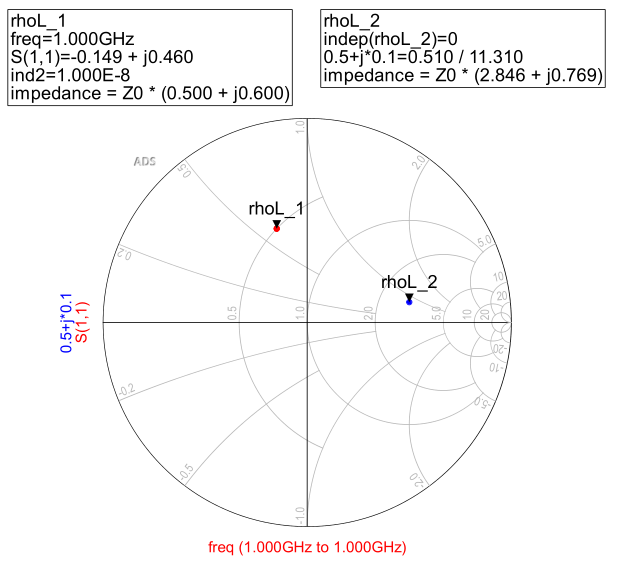
\includegraphics[width=9cm]{images/smith1.PNG}
\caption{Smith chart for the first half of problem 1.}
\label{p1:smith1} 
\end{figure}


The second half of the first problem issues the circuits of the figure \ref{p1:ckts}. In both it is asked to use a frequency of $1 GHz$ and to sweep the values of reactance. 

\begin{figure}[H] 
\centering
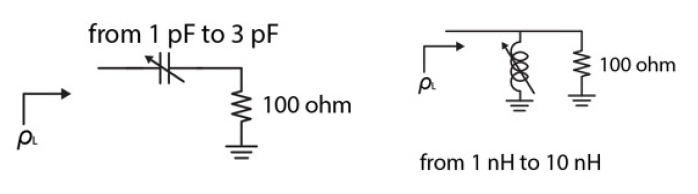
\includegraphics[width=10cm]{images/cktp1.png}
\caption{Circuits for problem 1.}
\label{p1:ckts} 
\end{figure}

The circuit at the left have a capacitor in series with a resistor, when varying the capacitance value, the Smith chart in figure \ref{p1:smith2} (a) will have the reflection coefficients varying in the circle of constant resistance. The figure \ref{p1:smith2} (b) show the same circuit for the admittance chart and it is clearly seen that the circuit behaviour is not easily observed by this kind of chart. 

\begin{figure}[H] 
\centering
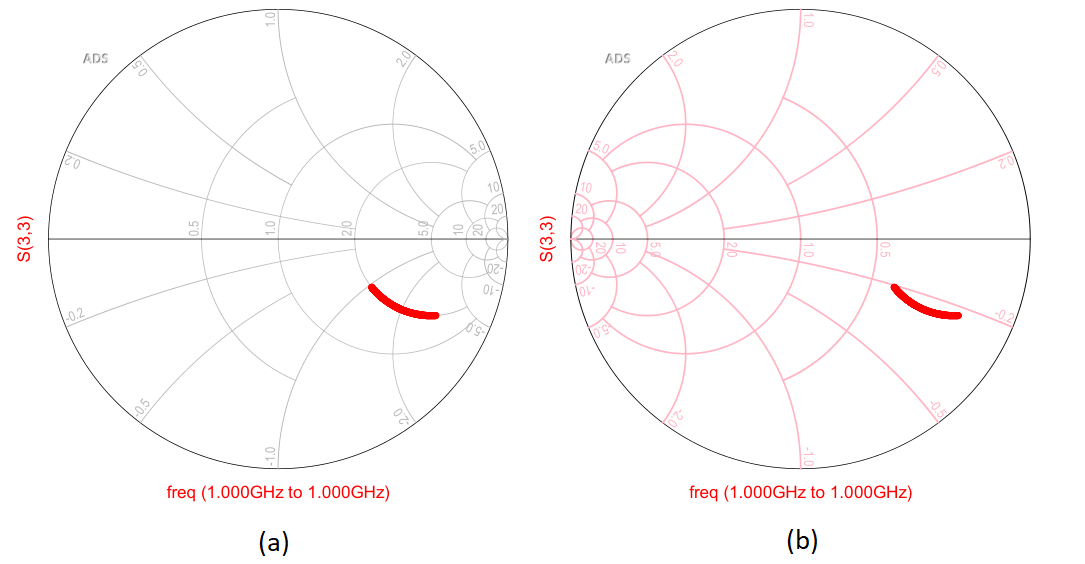
\includegraphics[width=15cm]{images/smith2.png}
\caption{Smith chart for the RC series circuit.}
\label{p1:smith2} 
\end{figure}

On the contrary, the circuit at the right have a inductance in parallel with a resistor and when varying the inductance, a most convenient way to observe the variation of the reflection coefficient is by the admittance chart in the figure \ref{p1:smith3} (a), since the markers walk in the circle of constant conductance.

\begin{figure}[H] 
\centering
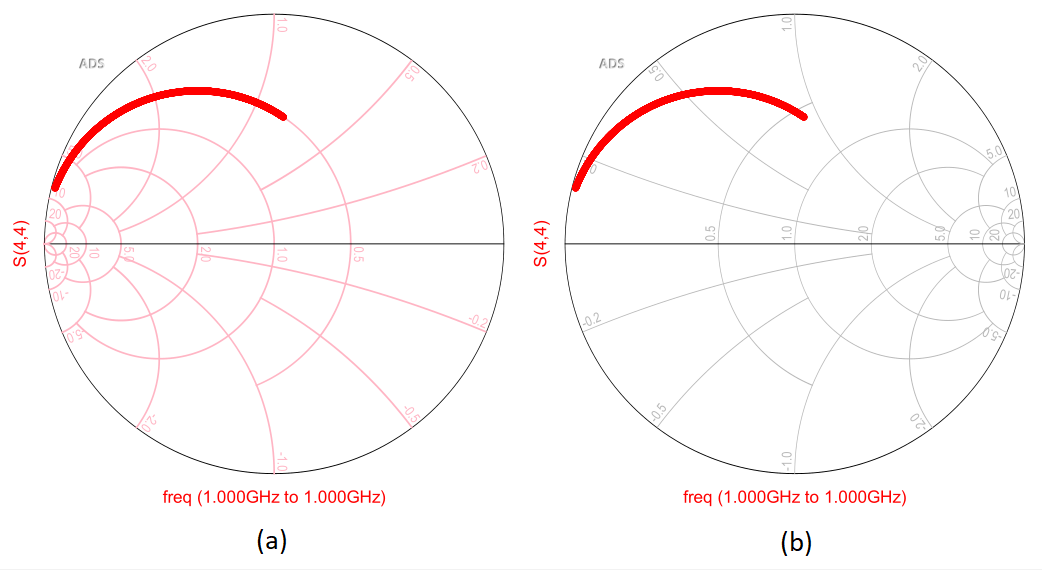
\includegraphics[width=15cm]{images/smith3.png}
\caption{Smith chart for the RL parallel circuit.}
\label{p1:smith3} 
\end{figure}